% This is "sig-alternate.tex" V2.1 April 2013
% This file should be compiled with V2.5 of "sig-alternate.cls" May 2012
%
% This example file demonstrates the use of the 'sig-alternate.cls'
% V2.5 LaTeX2e document class file. It is for those submitting
% articles to ACM Conference Proceedings WHO DO NOT WISH TO
% STRICTLY ADHERE TO THE SIGS (PUBS-BOARD-ENDORSED) STYLE.
% The 'sig-alternate.cls' file will produce a similar-looking,
% albeit, 'tighter' paper resulting in, invariably, fewer pages.
%
% ----------------------------------------------------------------------------------------------------------------
% This .tex file (and associated .cls V2.5) produces:
%       1) The Permission Statement
%       2) The Conference (location) Info information
%       3) The Copyright Line with ACM data
%       4) NO page numbers
%
% as against the acm_proc_article-sp.cls file which
% DOES NOT produce 1) thru' 3) above.
%
% Using 'sig-alternate.cls' you have control, however, from within
% the source .tex file, over both the CopyrightYear
% (defaulted to 200X) and the ACM Copyright Data
% (defaulted to X-XXXXX-XX-X/XX/XX).
% e.g.
% \CopyrightYear{2007} will cause 2007 to appear in the copyright line.
% \crdata{0-12345-67-8/90/12} will cause 0-12345-67-8/90/12 to appear in the copyright line.
%
% ---------------------------------------------------------------------------------------------------------------
% This .tex source is an example which *does* use
% the .bib file (from which the .bbl file % is produced).
% REMEMBER HOWEVER: After having produced the .bbl file,
% and prior to final submission, you *NEED* to 'insert'
% your .bbl file into your source .tex file so as to provide
% ONE 'self-contained' source file.
%
% ================= IF YOU HAVE QUESTIONS =======================
% Questions regarding the SIGS styles, SIGS policies and
% procedures, Conferences etc. should be sent to
% Adrienne Griscti (griscti@acm.org)
%
% Technical questions _only_ to
% Gerald Murray (murray@hq.acm.org)
% ===============================================================
%
% For tracking purposes - this is V2.0 - May 2012

\documentclass{sig-alternate-05-2015}


\begin{document}

% Copyright
\setcopyright{acmcopyright}
%\setcopyright{acmlicensed}
%\setcopyright{rightsretained}
%\setcopyright{usgov}
%\setcopyright{usgovmixed}
%\setcopyright{cagov}
%\setcopyright{cagovmixed}


% DOI
%\doi{10.475/123_4}

% ISBN
%\isbn{123-4567-24-567/08/06}

%Conference
%\conferenceinfo{PLDI '13}{June 16--19, 2013, Seattle, WA, USA}

%\acmPrice{\$15.00}

%
% --- Author Metadata here ---
%\conferenceinfo{WOODSTOCK}{'97 El Paso, Texas USA}
%\CopyrightYear{2007} % Allows default copyright year (20XX) to be over-ridden - IF NEED BE.
%\crdata{0-12345-67-8/90/01}  % Allows default copyright data (0-89791-88-6/97/05) to be over-ridden - IF NEED BE.
% --- End of Author Metadata ---

\title{Ease the Process of Machine Learning with Dataflow}
%\subtitle{[Extended Abstract]
%\titlenote{A full version of this paper is available as
%\textit{Author's Guide to Preparing ACM SIG Proceedings Using
%\LaTeX$2_\epsilon$\ and BibTeX} at
%\texttt{www.acm.org/eaddress.htm}}}
%
% You need the command \numberofauthors to handle the 'placement
% and alignment' of the authors beneath the title.
%
% For aesthetic reasons, we recommend 'three authors at a time'
% i.e. three 'name/affiliation blocks' be placed beneath the title.
%
% NOTE: You are NOT restricted in how many 'rows' of
% "name/affiliations" may appear. We just ask that you restrict
% the number of 'columns' to three.
%
% Because of the available 'opening page real-estate'
% we ask you to refrain from putting more than six authors
% (two rows with three columns) beneath the article title.
% More than six makes the first-page appear very cluttered indeed.
%
% Use the \alignauthor commands to handle the names
% and affiliations for an 'aesthetic maximum' of six authors.
% Add names, affiliations, addresses for
% the seventh etc. author(s) as the argument for the
% \additionalauthors command.
% These 'additional authors' will be output/set for you
% without further effort on your part as the last section in
% the body of your article BEFORE References or any Appendices.

\numberofauthors{1} %  in this sample file, there are a *total*
% of EIGHT authors. SIX appear on the 'first-page' (for formatting
% reasons) and the remaining two appear in the \additionalauthors section.
%
\author{
% You can go ahead and credit any number of authors here,
% e.g. one 'row of three' or two rows (consisting of one row of three
% and a second row of one, two or three).
%
% The command \alignauthor (no curly braces needed) should
% precede each author name, affiliation/snail-mail address and
% e-mail address. Additionally, tag each line of
% affiliation/address with \affaddr, and tag the
% e-mail address with \email.
%
% 1st. author
\alignauthor
Tianyou Guo, Jun Xu\thanks{Jun Xu is the corresponding author}, Xiaohui Yan\thanks{Current affiliation: DiDi Research, Beijing}, Jianpeng Hou, \\Ping Li, Zhaohui Li, Jiafeng Guo, Xueqi Cheng\\
       \affaddr{CAS Key Laboratory of Network Data Science and Technology, Institute of Computing Technology, CAS}\\
       \email{\{guotianyou, houjianpeng, liping, lizhaohui\}@software.ict.ac.cn, \\ \{junxu, yanxiaohui, guojiafeng, cxq\}@ict.ac.cn}
}
\maketitle
\begin{abstract}
Machine learning algorithms have become the key components in many big data applications. However, the full potential of machine learning is still far from been realized because using machine learning algorithms is hard, especially on distributed platforms such as Hadoop~\cite{Hadoop} and Spark~\cite{zaharia2010spark,Spark}. The key barriers come from not only the implementation of the algorithms themselves, but also the processing for applying them to real applications which often involve multiple steps and different algorithms. In this demo we present a general-purpose dataflow-based system for easing the process of applying machine learning algorithms to real world tasks. In the system, a learning task is formulated as a directed acyclic graph (DAG) in which each node represents an operation (e.g., a machine learning algorithm), and each edge represents the flow of the data from one node to its descendants. The task can be defined manually or be cloned from existing tasks/templates. After submitting a task to the cloud, each node will be automatically scheduled to execute according to the DAG. Graphical user interface is implemented for making users to create, configure, submit, and monitor a task in a drag-and-drop manner. Advantages of the system include 1) lowing the barriers of defining and executing machine learning tasks; 2) sharing and re-using the implementations of the algorithms, the job DAGs, and the (intermediate) experimental results; 3) seamlessly integrating the stand-alone algorithms as well as the distributed algorithms in one task. The system has been deployed as a machine learning service in Institute of Computing Technology, Chinese Academy of Sciences and can be access from the Internet.
\end{abstract}


%\keywords{Machine learning process; dataflow, directed acyclic graph}

\section{Introduction}
Machine learning has become the core of many big data applications such as information retrieval, question answering, and recommender system etc. To fulfill the increasing requirements on machine learning algorithms, a number of scalable machine learning libraries, including Apache Mahout~\cite{Mahout} and Spark MLlib~\cite{SparkMLLib}, have been released and widely used. Despite the widespread impacts of the machine learning libraries, it is still difficult for ordinary users to use the machine learning in their applications. The barrier mainly comes from the complex process of using machine learning algorithms to solve a real-world task. A supervised learning task usually consists of multiple steps including data preparation, feature extraction, model training, testing, and performance evaluation etc. The process could become more complicated if multiple learning algorithms and datasets are involved. For example, the user may want to use the topics as features in the task of document categorization. Thus, the process need to first train a topic model based on some dataset, and then feed the learned topics to a classification model~\cite{XXX}. It has been widely recognized that constructing an appropriate process is crucial for the success of applying machine learning to real world application. Therefore, a platform that can help ease the construction and running process will be of great help to users.

In this demo, we present a general-purpose machine learning system for lowering the barrier to applying machine learning algorithms. In the system, we consider the process of applying machine learning algorithms from the viewpoint of dataflow. Thus, the process can be formulated as a directed acyclic graph (DAG) in which the source data flow into the root nodes. Each node makes operations on the data, generates new data, and sends the generated data to its descendant nodes for conducting further operations. Finally, the results flow out from the leaf nodes.

The system consists of three major components: 1) A distributed machine learning library which implements not only popular used machine learning algorithms, but also the algorithms for data pre/post-processing, data format transformation, feature generation, performance evaluation etc. These algorithms are mainly implemented based on Spark.  2) A GUI-based machine learning studio which enable users to create, configure, submit, monitor, and share their machine learning process in a drag-and-drop manner. All of the algorithms in the machine learning library can be accessed and configured in the studio. They are the key building blocks for constructing machine learning tasks. 3) A cloud service for executing the tasks. We build the service based on the open source big data platform of Hadoop and Spark. After receiving a task DAG from the GUI, each node will be automatically scheduled to run when all of its dependent data sources are ready. The algorithm corresponds to the node will scheduled to run on Linux, Spark, or Map-Reduce~\cite{dean2004mapreduce,dean2010mapreduce}, according to their implementation.

The system offers several distinct advantages for applying machine learning to real tasks: 1) The dataflow formulation of machine learning tasks is quite intuitive and easy to understand. The GUI hides the unnecessary technical details of the algorithms (e.g., the complex command line) and helps user to focus on building the task process; 2) Users can upload and share their own algorithms and data to the system. They can also share their historical tasks to other users. In this way, a new task can be created easily by cloning and making minor modifications. To save the execution time and computational resource, the results generated by existing tasks can be reused by other tasks; 3) It has the ability to use the stand-alone algorithms, Spark algorithms, and Map-Reduce algorithms in one DAG. Ordinary users can use and configure the distributed algorithms in the same way as that of the stand-alone algorithms.

Several similar systems have been developed and released in enterprise and open source community. Mahout and MLlib are two distributed machine learning libraries developed with Hadoop Map-Reduce and Spark, respectively. A number of popular machine learning algorithms have been implemented in the libraries. To make these algorithms working together, people considers the application of machine learning as a workflow and several workflow schedulers have been developed, including the open source systems of Oozie~\cite{islam2012oozie,Oozie}, HUE~\cite{HUE}, and Azkaban~\cite{Azkaban} etc. Microsoft has also released Azure machine learning~\cite{barga2014introducing,AzureML} in which a machine learning process is formalized as a dataflow. Azure machine learning is built on the cloud computing platform Microsoft Azure and provide machine learning service in the cloud.

In the following sections, we first introduce the dataflow formalization of the machine learning process, followed by the system architecture and core technologies used in the system. Finally, we give the demonstration plan.

\section{Machine Learning Process as a Dataflow DAG}
A typical application of the machine learning algorithms consists of several steps include gathering and preprocessing the data, extracting features, applying the training algorithm, and testing the performances of the trained model. From the viewpoint of data, the whole process can be viewed as the raw data flow into the processing pipeline. After a number of step-by-step operations on the data, the result data flow out the pipeline. The process could be much more complex if multiple machine learning algorithms are involved.

Our system formulates the complex process of applying machine learning algorithms as a DAG of dataflow in which the data flows in the graph according to the directed edges. The data will be processed by the nodes it flows through. Each node consists of several input ports, output ports, and an operation. Each input port corresponds to an flow in data file and each output port corresponds to a data file that flows out. The operation is a (stand-alone or distributed) program that reads the input ports and writes the results to output ports. In our system, the operation of each node is implemented as a Linux command line. A dataflow DAG may also contain some data nodes which represent the input data sources. Please note that a data node only have one output port. Figure~\ref{fig:dag} shows a typical dataflow DAG of applying the machine learning algorithm of random forest for binary classification. Different colors are used to show the different status of the nodes: green for success, yellow for under executing, gray for waiting, and red for failed.
\begin{figure}
\centering
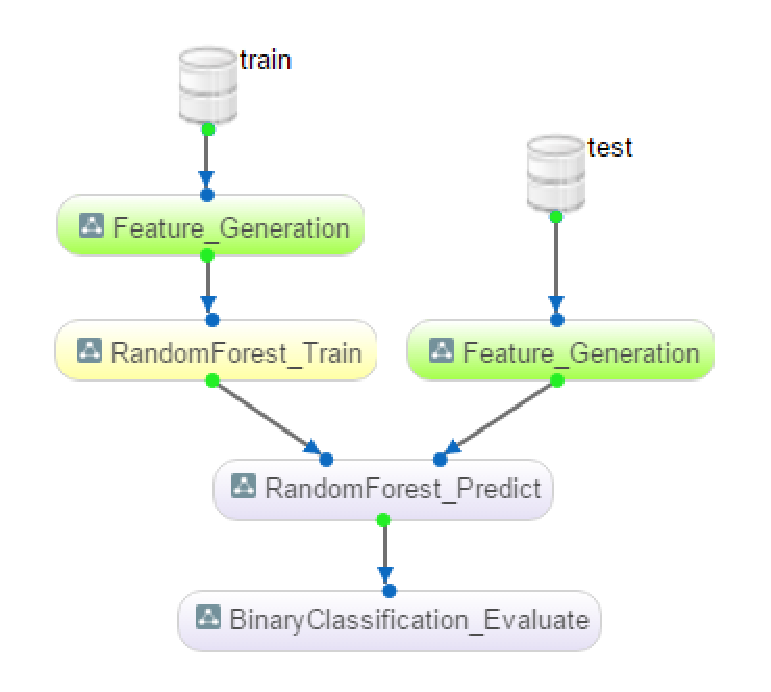
\includegraphics[width = 0.3\textwidth]{DAG.eps}
\caption{An example dataflow DAG.}
\label{fig:dag}
\end{figure}

\section{System Overview}
%\subsection{System Architecture}
Figure~\ref{fig:arch} shows the architecture of the our system. The whole system consists of three parts: big data infrastructure for providing the foundation services, machine learning library for providing the core building blocks of the machine learning tasks, and machine learning studio for providing user-friendly GUI to lower the barrier of using machine learning.

\begin{figure}[t]
\centering
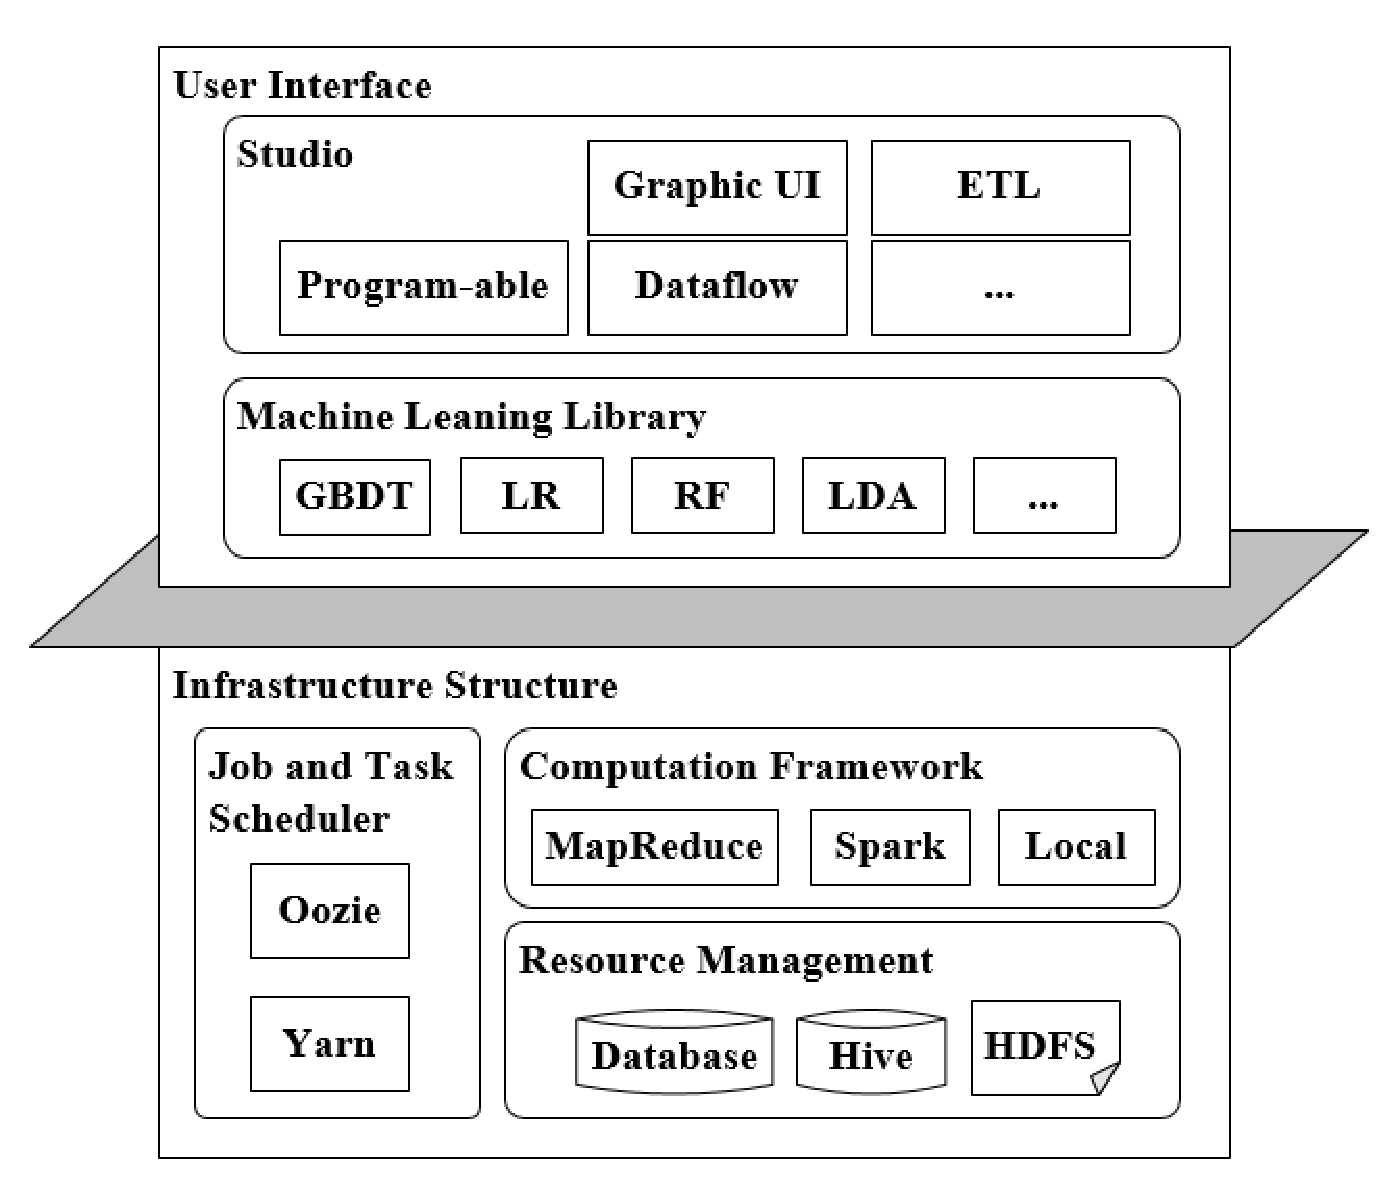
\includegraphics[width=0.4\textwidth]{arch.eps}
\caption{ An overview of system architecture.}
\label{fig:arch}
\end{figure}

\noindent\textbf{Big Data Infrastructure}

Our system is built upon the open source big data system of Hadoop and Spark. All the data, machine learning algorithms, and other dependent information are stored in the distributed file system HDFS and data management system of Hive. A relational database system of MySQL is used for storing the metadata. Our system also depend on the distributed computational framework of Map-Reduce and Spark. All of the computational resources are managed with Yarn. Each of the submitted machine learning task (a dataflow DAG) is first converted to a workflow DAG and scheduled with the workflow scheduler system Oozie.

\noindent\textbf{Machine learning library}

The machine learning library implements a number of popular machine learning algorithms (e.g., classification, topic modeling, graph processing, and information recommendation etc). For each algorithm, we implemented the distributed version on Spark as well as the standalone version because the standalone versions are usually more efficient than the distributed versions if the datasets are not big enough. Besides the core algorithms, the library also implements necessary modules for supporting the core algorithms including data pre/post-processing, data format transformation, feature extraction, and performance evaluation etc. All of the algorithms and modules can be called via both the Linux command line and Java API. These algorithms constitute the core building blocks for users to define their machine learning tasks.


\noindent\textbf{Machine learning studio}

The main goal of the machine learning studio is to provide a user-friendly GUI so that ordinary users can use the machine learning algorithms to solve their own problems easily. The machine learning studio is implemented as a web service and can be accessed via web browsers. It provides the follow main features:

(1) \textbf{Resource management}: All algorithms implemented in the machine learning library can be accessed from the studio system. The system also provide a a number of data and tasks for showing how to use the algorithms to solve a problem. To construct a machine learning task, users may directly use the algorithms and data in the system. They can also upload their own data and algorithm packages. To upload an algorithm package, the user need to specify the format of the Linux command line string for running the algorithm. The string defines the program name, the input data, the output data, and the parameters. In a specified task dataflow DAG, the algorithm can be scheduled to run according to the command line. After a machine learning task is submitted, it will be assigned a unique ID and stored in the task repository. Users can check and reuse the task in the future. They can also share the task to other users.

(2) \textbf{Task design}: To construct a machine learning task, a user may drag the algorithms and data sets (nodes) to the work panel, connect these nodes as a dataflow DAG, and set the parameters of all the nodes. If the users can find a similar task in our repository (in most cases), they can directly clone an existing task and make necessary modifications (add/remove nodes and edges, change parameters). By selecting a node in the work panel, the parameter setting panel will be shown in the right part of the page, which enables the users to set the specific parameter values for the corresponding algorithm in the task. After submitting a machine learning task, the studio will check the correctness of the dataflow DAG, generate the file paths of the temporal files, convert dataflow DAG to a work-flow DAG, and finally submit the work-flow DAG to Oozie for execution.

(3) \textbf{Task monitoring}: Users can monitor the progresses of a submitted task through the studio. During the execution of a task, different colors are used to indicate the status of the nodes: green for completed successfully, yellow for under running, red for completed with errors, and gray for waiting to execute. The results of a success node can be checked and downloaded via right clicking the corresponding output ports. The information printed to the standard out and standard error consoles can also be checked by right clicking the corresponding nodes. Through this way, users can know the status of a task and debug their algorithms and tasks if any error occurs.

(4) \textbf{Task Reusing}: An existing task can not only be used as templates for designing new tasks but also be reused for saving the execution time and system resource. Users may directly modify a completed task (e.g., modify the parameters of the nodes, add nodes and edges, or delete nodes and edges etc.) and resubmit the task. In the newly submitted task, only the influenced nodes are scheduled to execute and the results outputted by the uninfluenced nodes will be reused directly. For solving a real task, users usually need to tune their task dataflow DAG and parameters of the algorithms over and over. Task re-usage provides us an effective and efficient mechanism to save the user waiting time and system resources.


\section{Advantages}
Our system offers the following advantages.

1) It is an easy-to-use and quite powerful system. The dataflow DAG formulation of the machine learning task is intuitive and easy to understand for ordinary users. Many unnecessary details are hidden. On the other hand, it still provides a lot of details (e.g., the parameters settings, the input/output ports etc.) for expert users.

2) The system seamlessly integrates the heterogeneous programs in one task. Since we used the HDFS for exchanging the information across different nodes, we have very few restriction on the form of the programs for the DAG nodes. The program corresponds to a node could be executed in stand-alone or distributed manner. It could be written with the programming language of C++, Java, Python, Perl or even the shell language.

3) The data, algorithms, and tasks in the system are highly reusable. Users can make use of the data and algorithms developed our library for constructing different machine learning tasks. The can also make use of the data and algorithms uploaded/shared by other users. A task can be cloned to construct similar tasks. Moreover, the intermediate results of an existing task can be reused by modifying and appending the task directly.


\section{Demo Plan}
We will present our system in the following aspects: First, we will use a poster to give an overview of system architecture and briefly show the dataflow DAG formulation of the machine learning tasks and the system components.
Next, we will show the audience how to use the system to complete a example machine learning task, including creating, configuring, submitting, and monitoring a task.After that, we will show the algorithms and datasets in the system. We will also show advanced functions of the system such as uploading new algorithms and datasets, sharing and reusing existing tasks etc. The audience will gain a deeper understanding on the system.Finally, we will share our thoughts on the strengths and weakness of the system. We will further discuss future work.

\bibliographystyle{abbrv}
\bibliography{sigproc}

%ACKNOWLEDGMENTS are optional
\newpage
%APPENDICES are optional
%\balancecolumns
\appendix

%Appendix A

Online system URL is http://159.226.40.104:18080/studio/. 
If you don't want to register an account, please use account \textbf{bdaict@hotmail.com}, the password is \textbf{bdaict}.

\noindent\textbf{System Home Page}

An user of our system must register or login firstly from the home page showed as follow:
\begin{figure}[!htb]
\centering

\includegraphics[width = 0.4\textwidth]{HomePage.eps}
\end{figure}

\noindent\textbf{An Example of Machine Learning Job}

We support drag-and-drop manner of machine learning job construction. The parameters and informations of the job is also configurable from UI page. Shown as follow:
\begin{figure}[!htb]
\centering
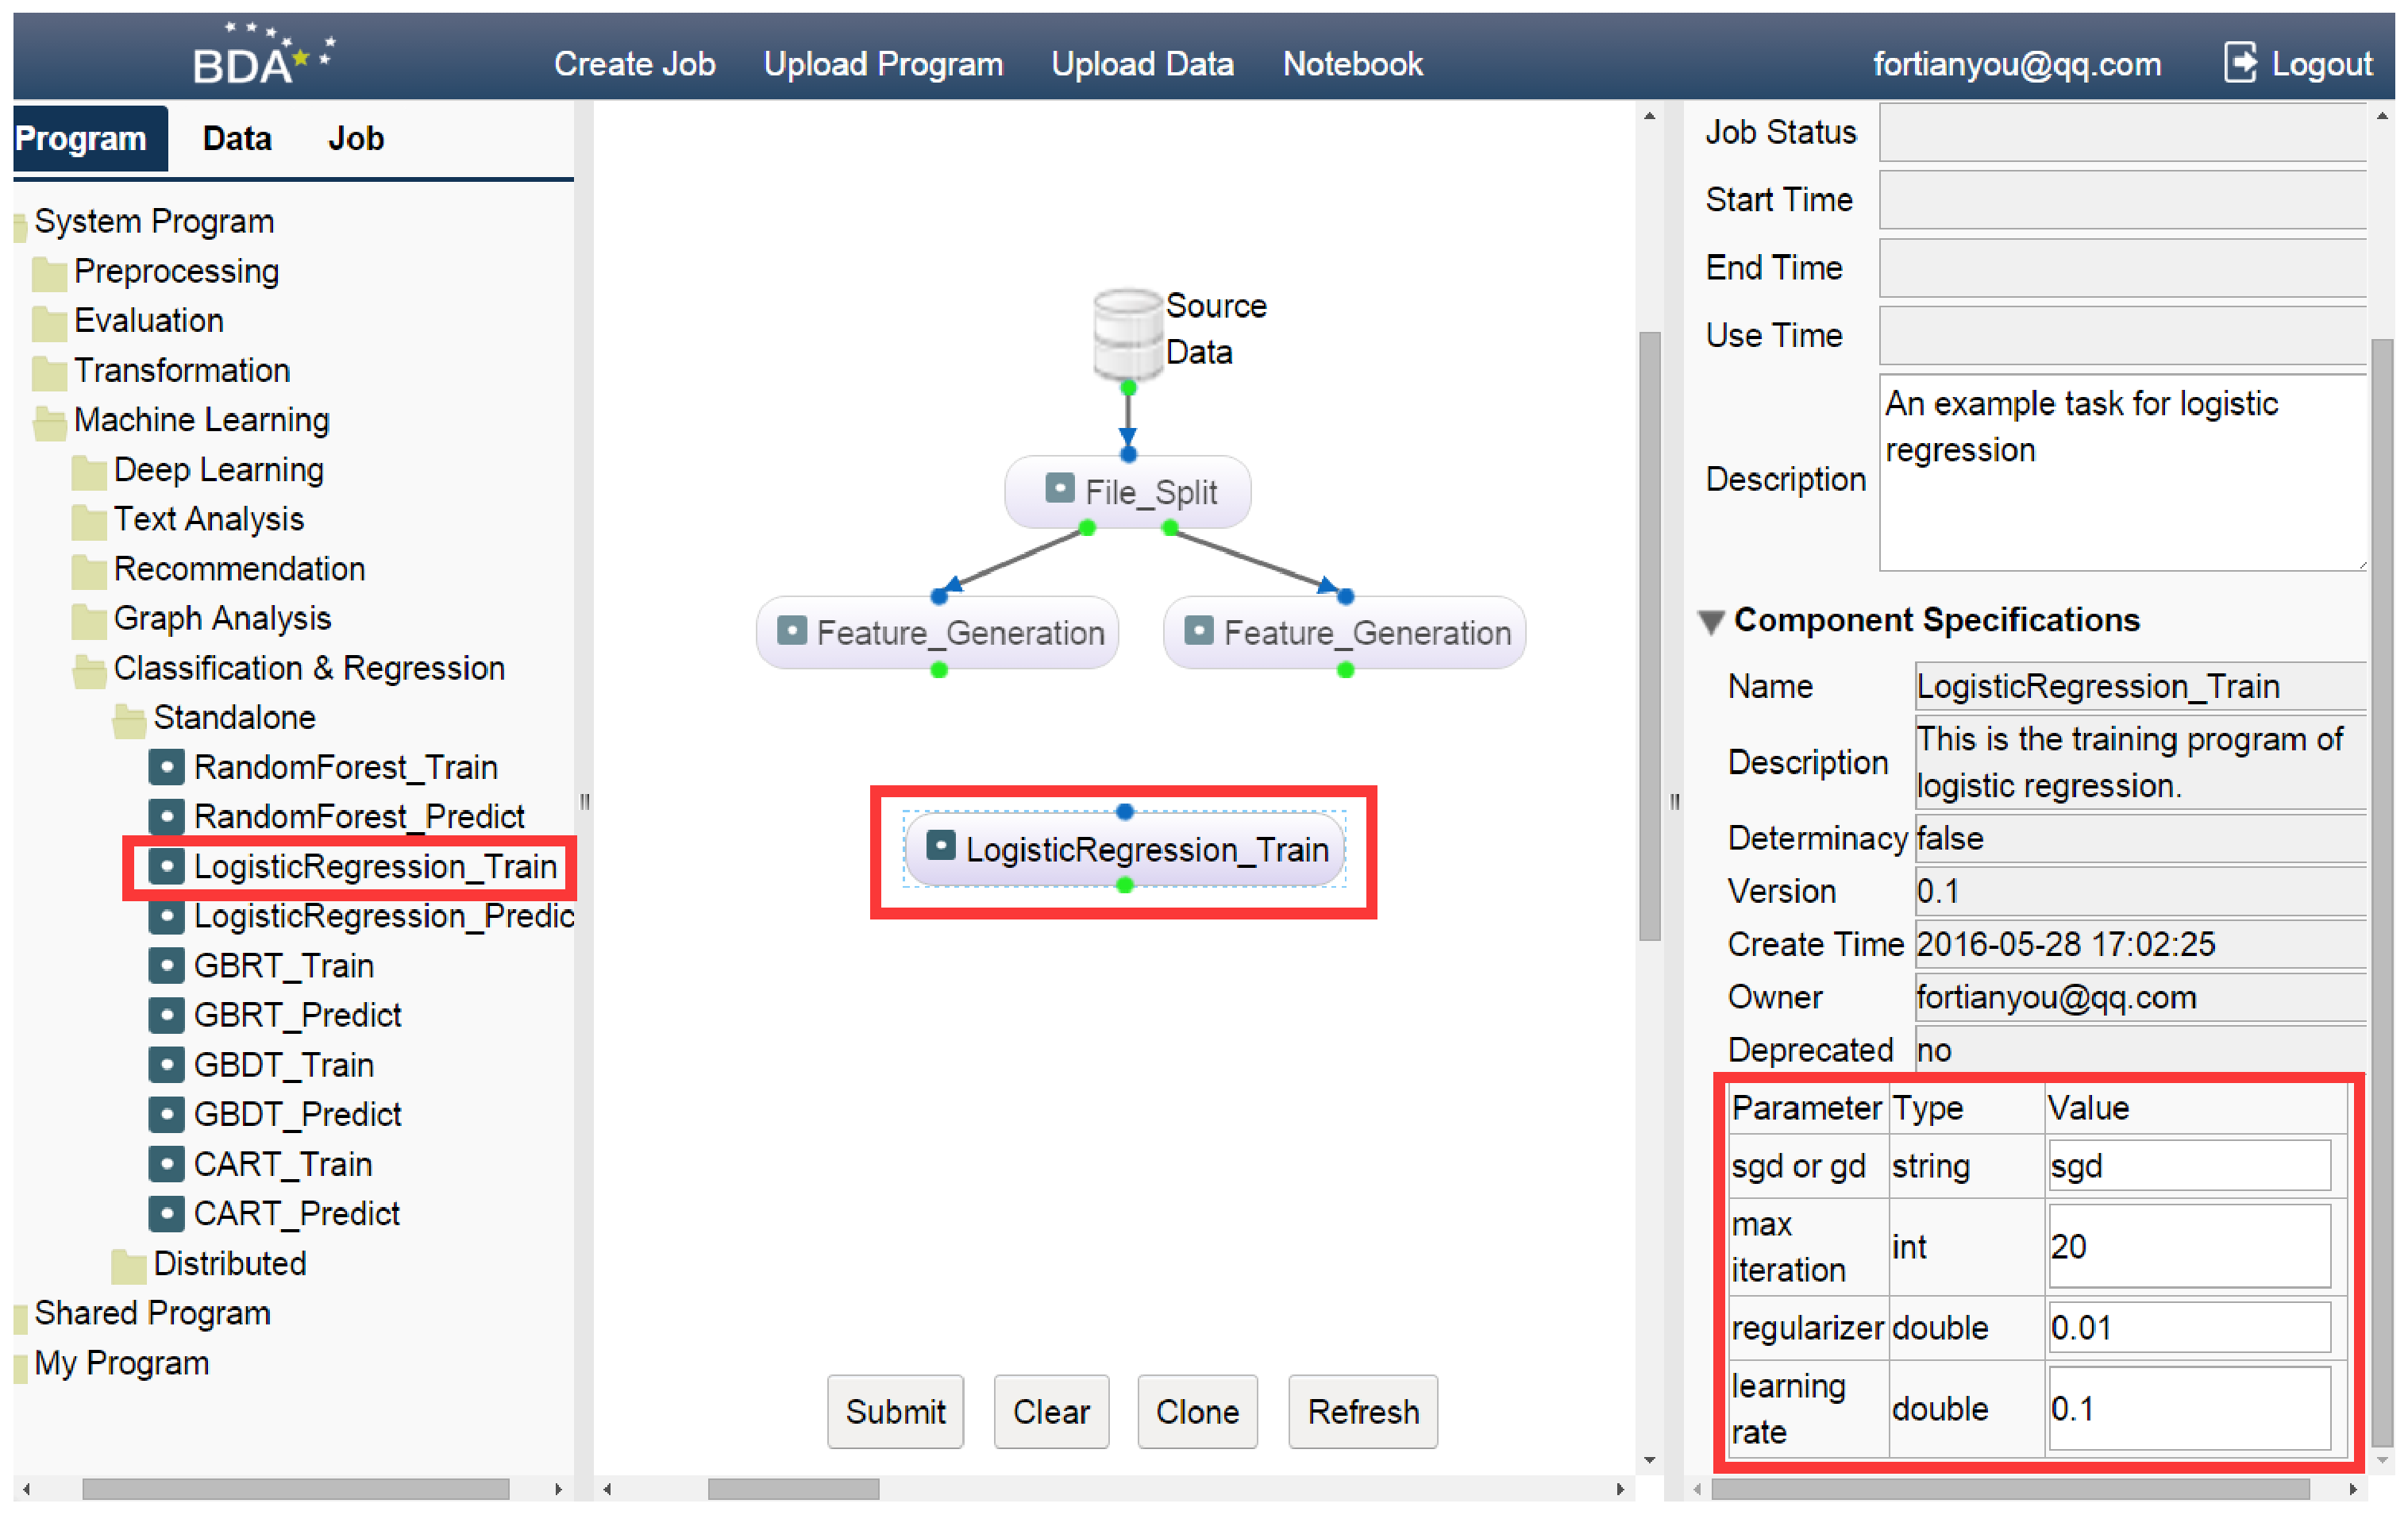
\includegraphics[width = 0.4\textwidth]{job_construct.eps}
\end{figure}

After dataflow DAG is well configured, please click "submit" button to submit and run the job. As is shown, the job is running:

\begin{figure}[!htb]
\centering
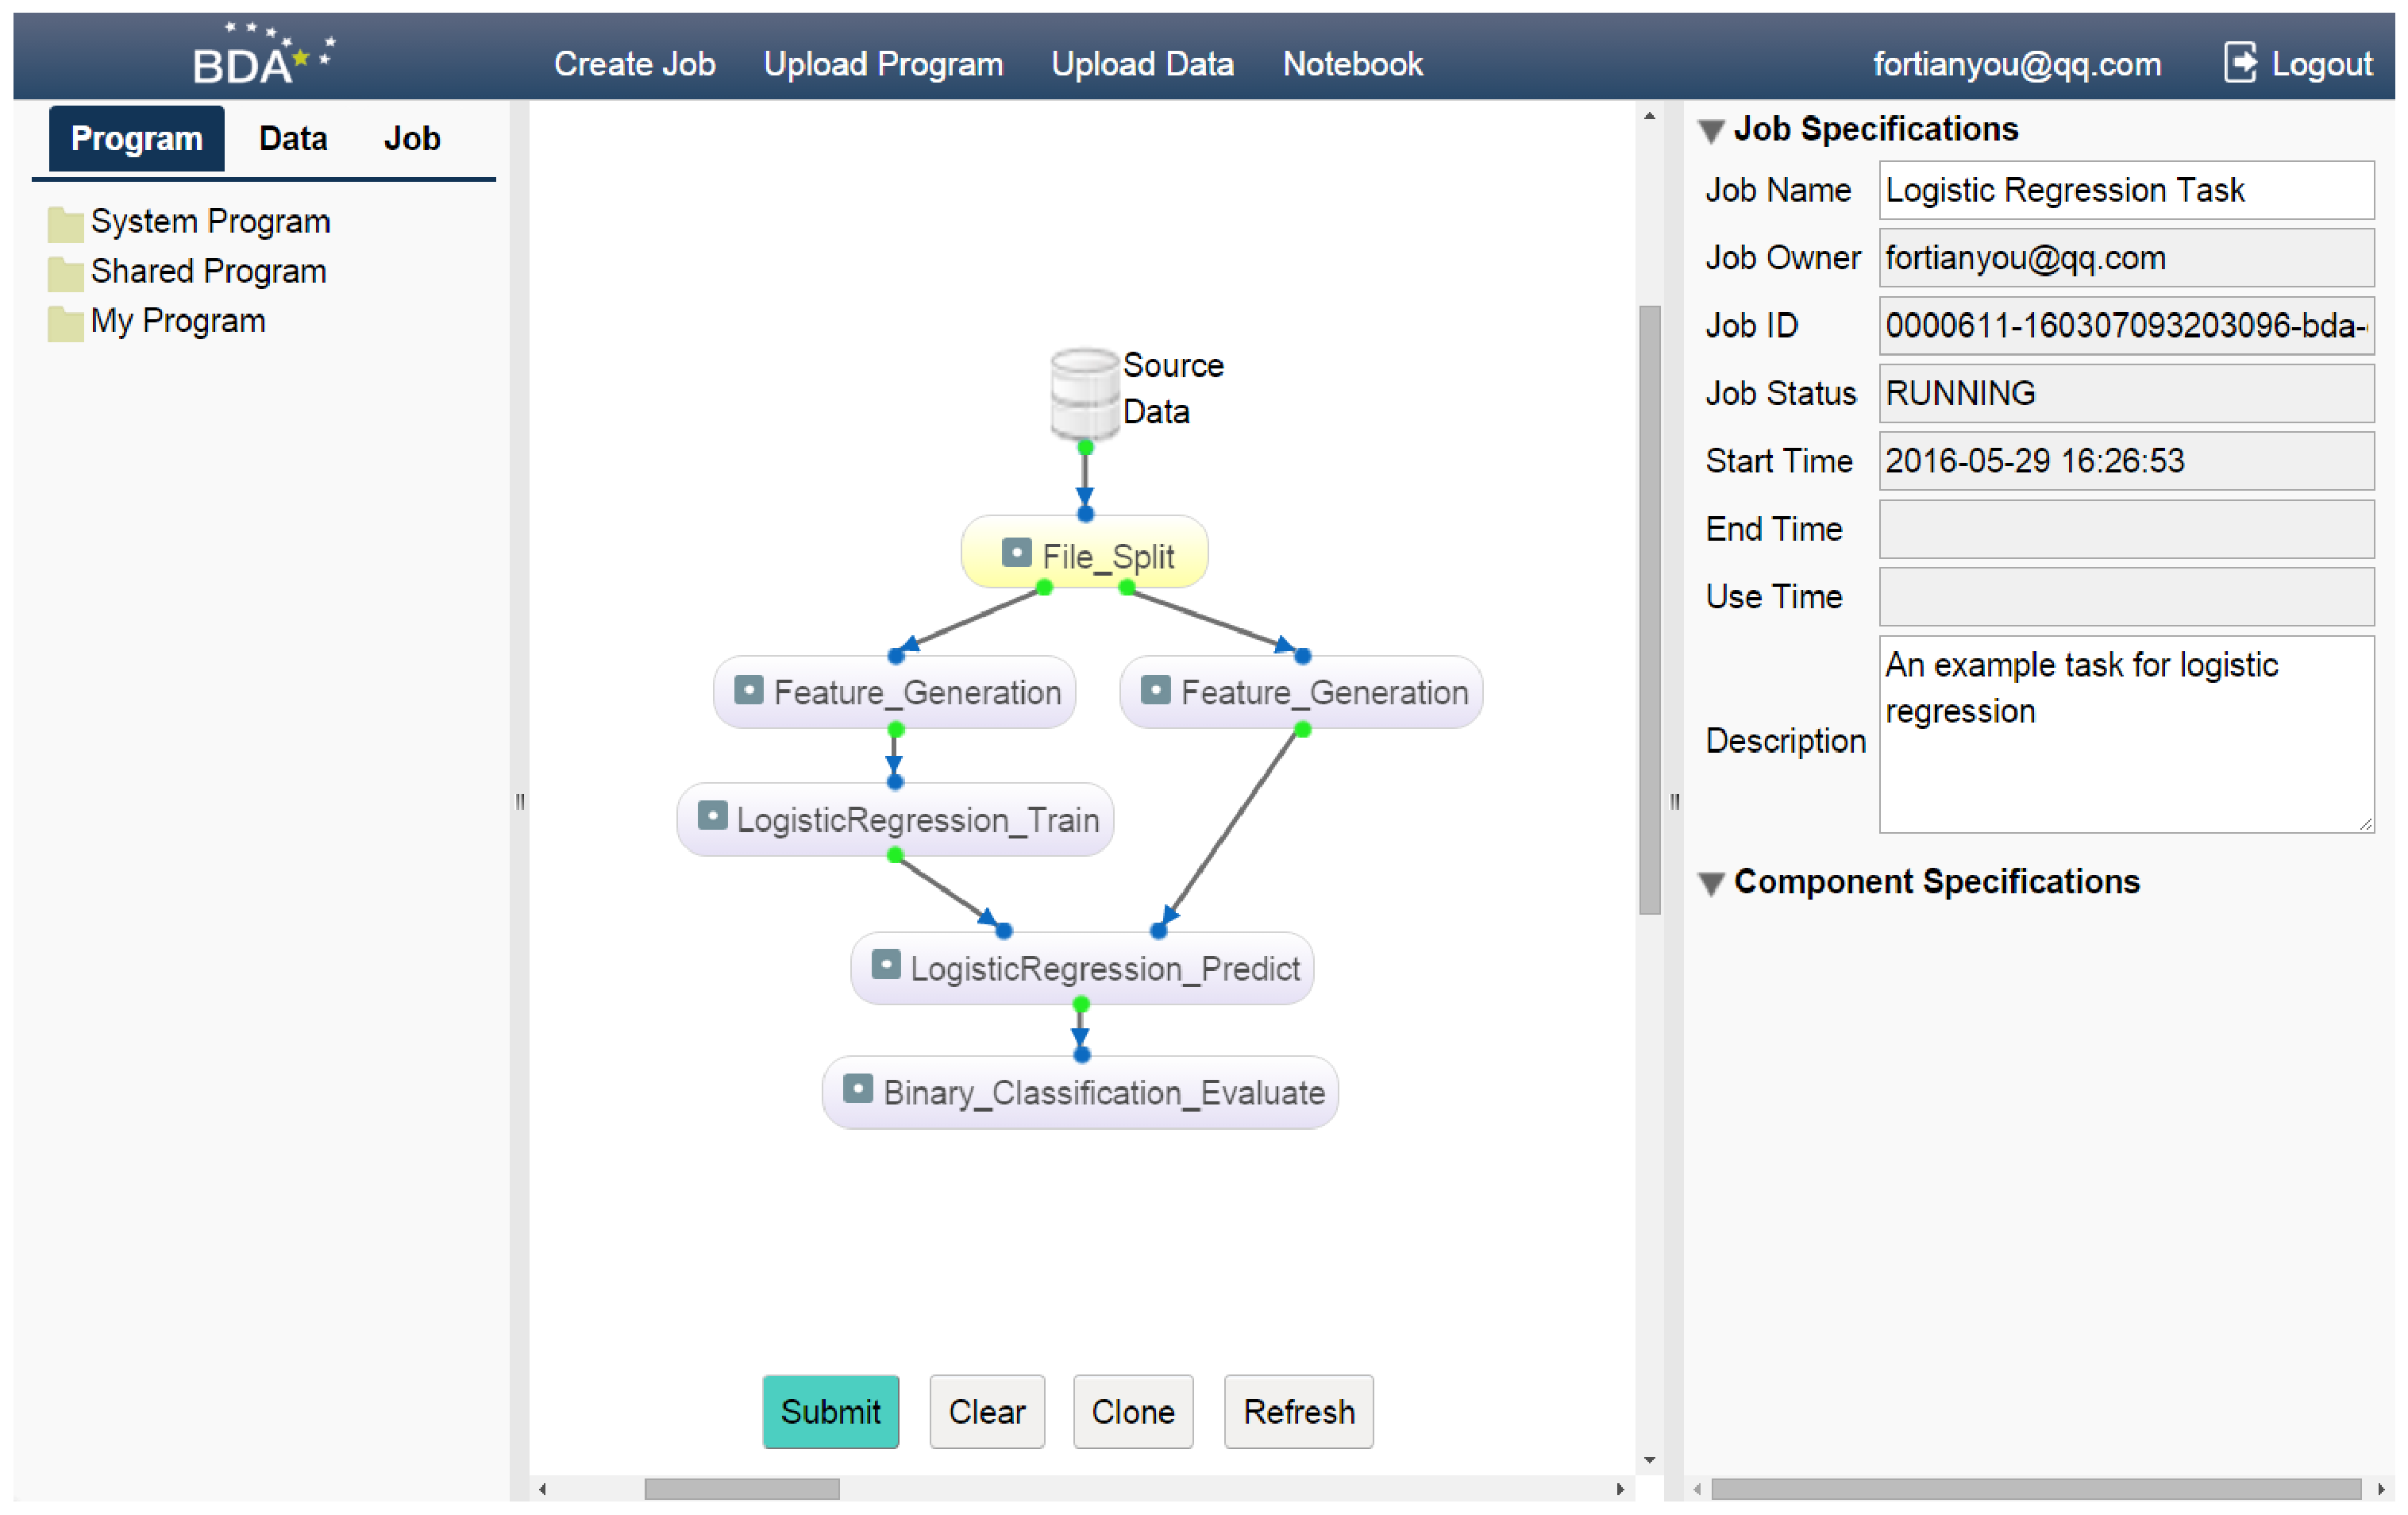
\includegraphics[width = 0.4\textwidth]{job_submit.eps}
\end{figure}

One could right click on the green output port of finished executing node to preview the output data. One could check the stdout and stderr logs from the right click menu of each finished executing node as well.

\begin{figure}[!htb]
\centering
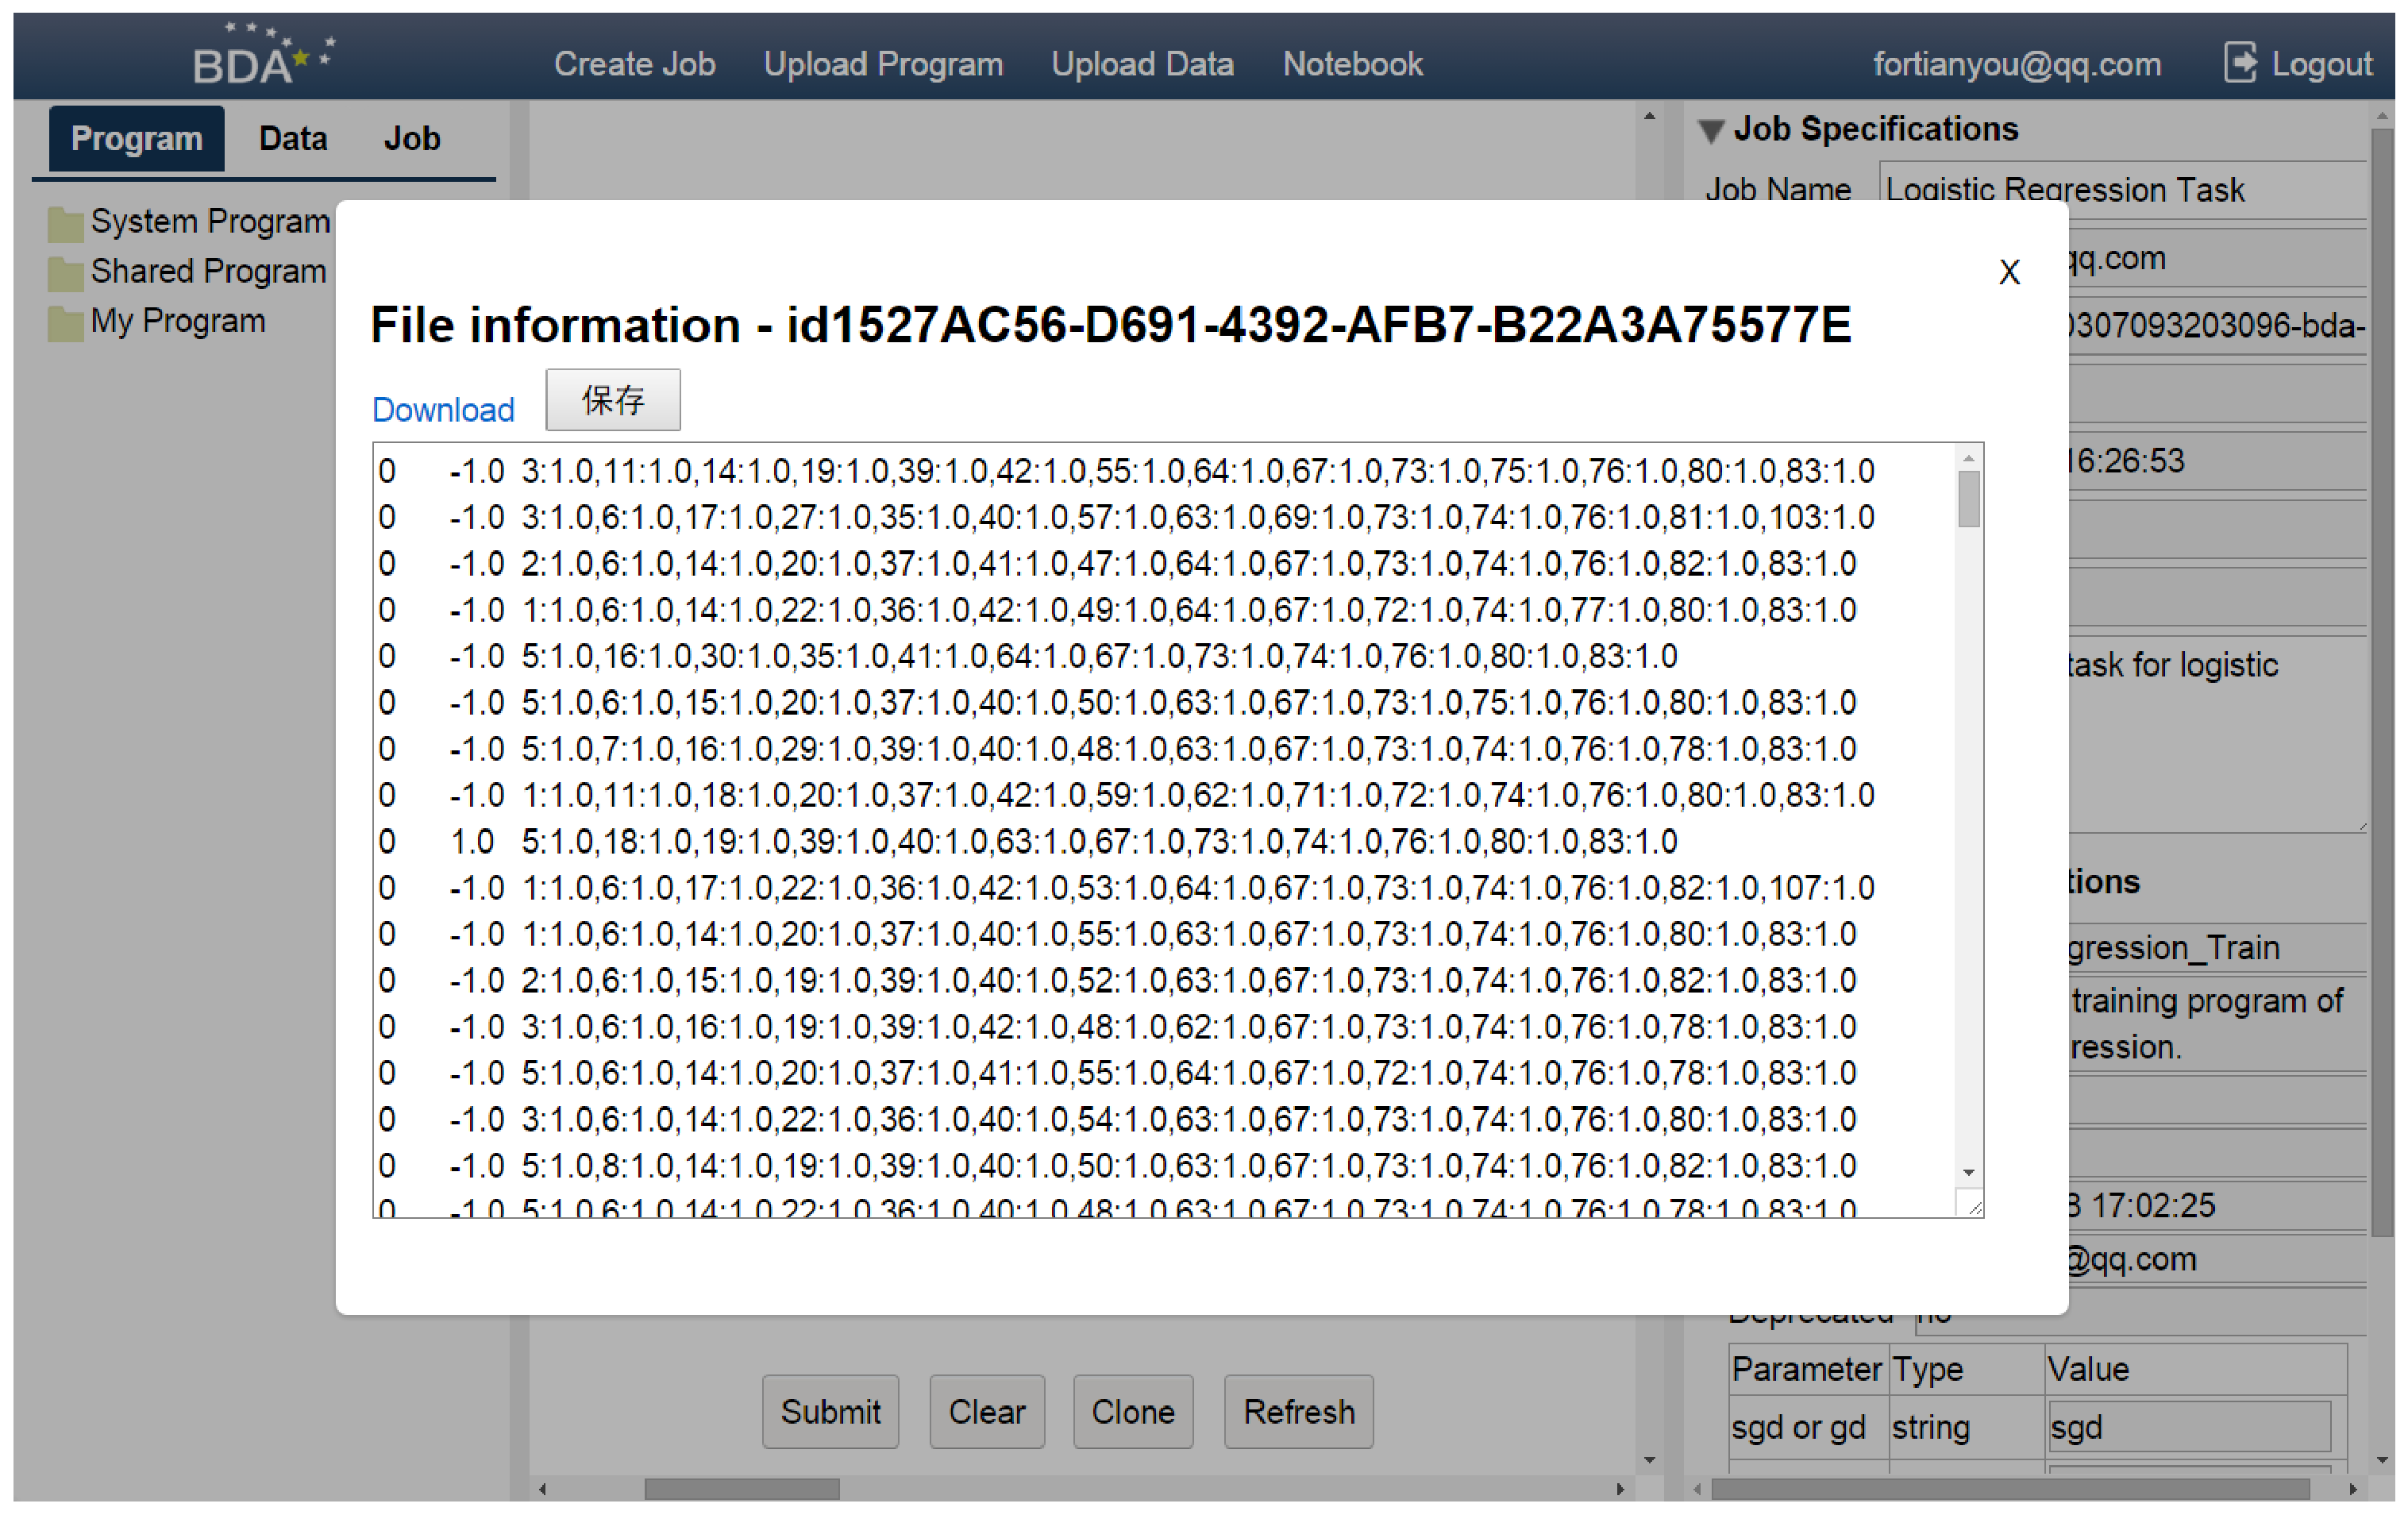
\includegraphics[width = 0.4\textwidth]{job_data_output.eps}
\end{figure}

When the job is finished, one is enable to modify and append operations to the job. As is shown bellow, we had add some new operation node into the dataflow DAG:

\begin{figure}[!htb]
\centering
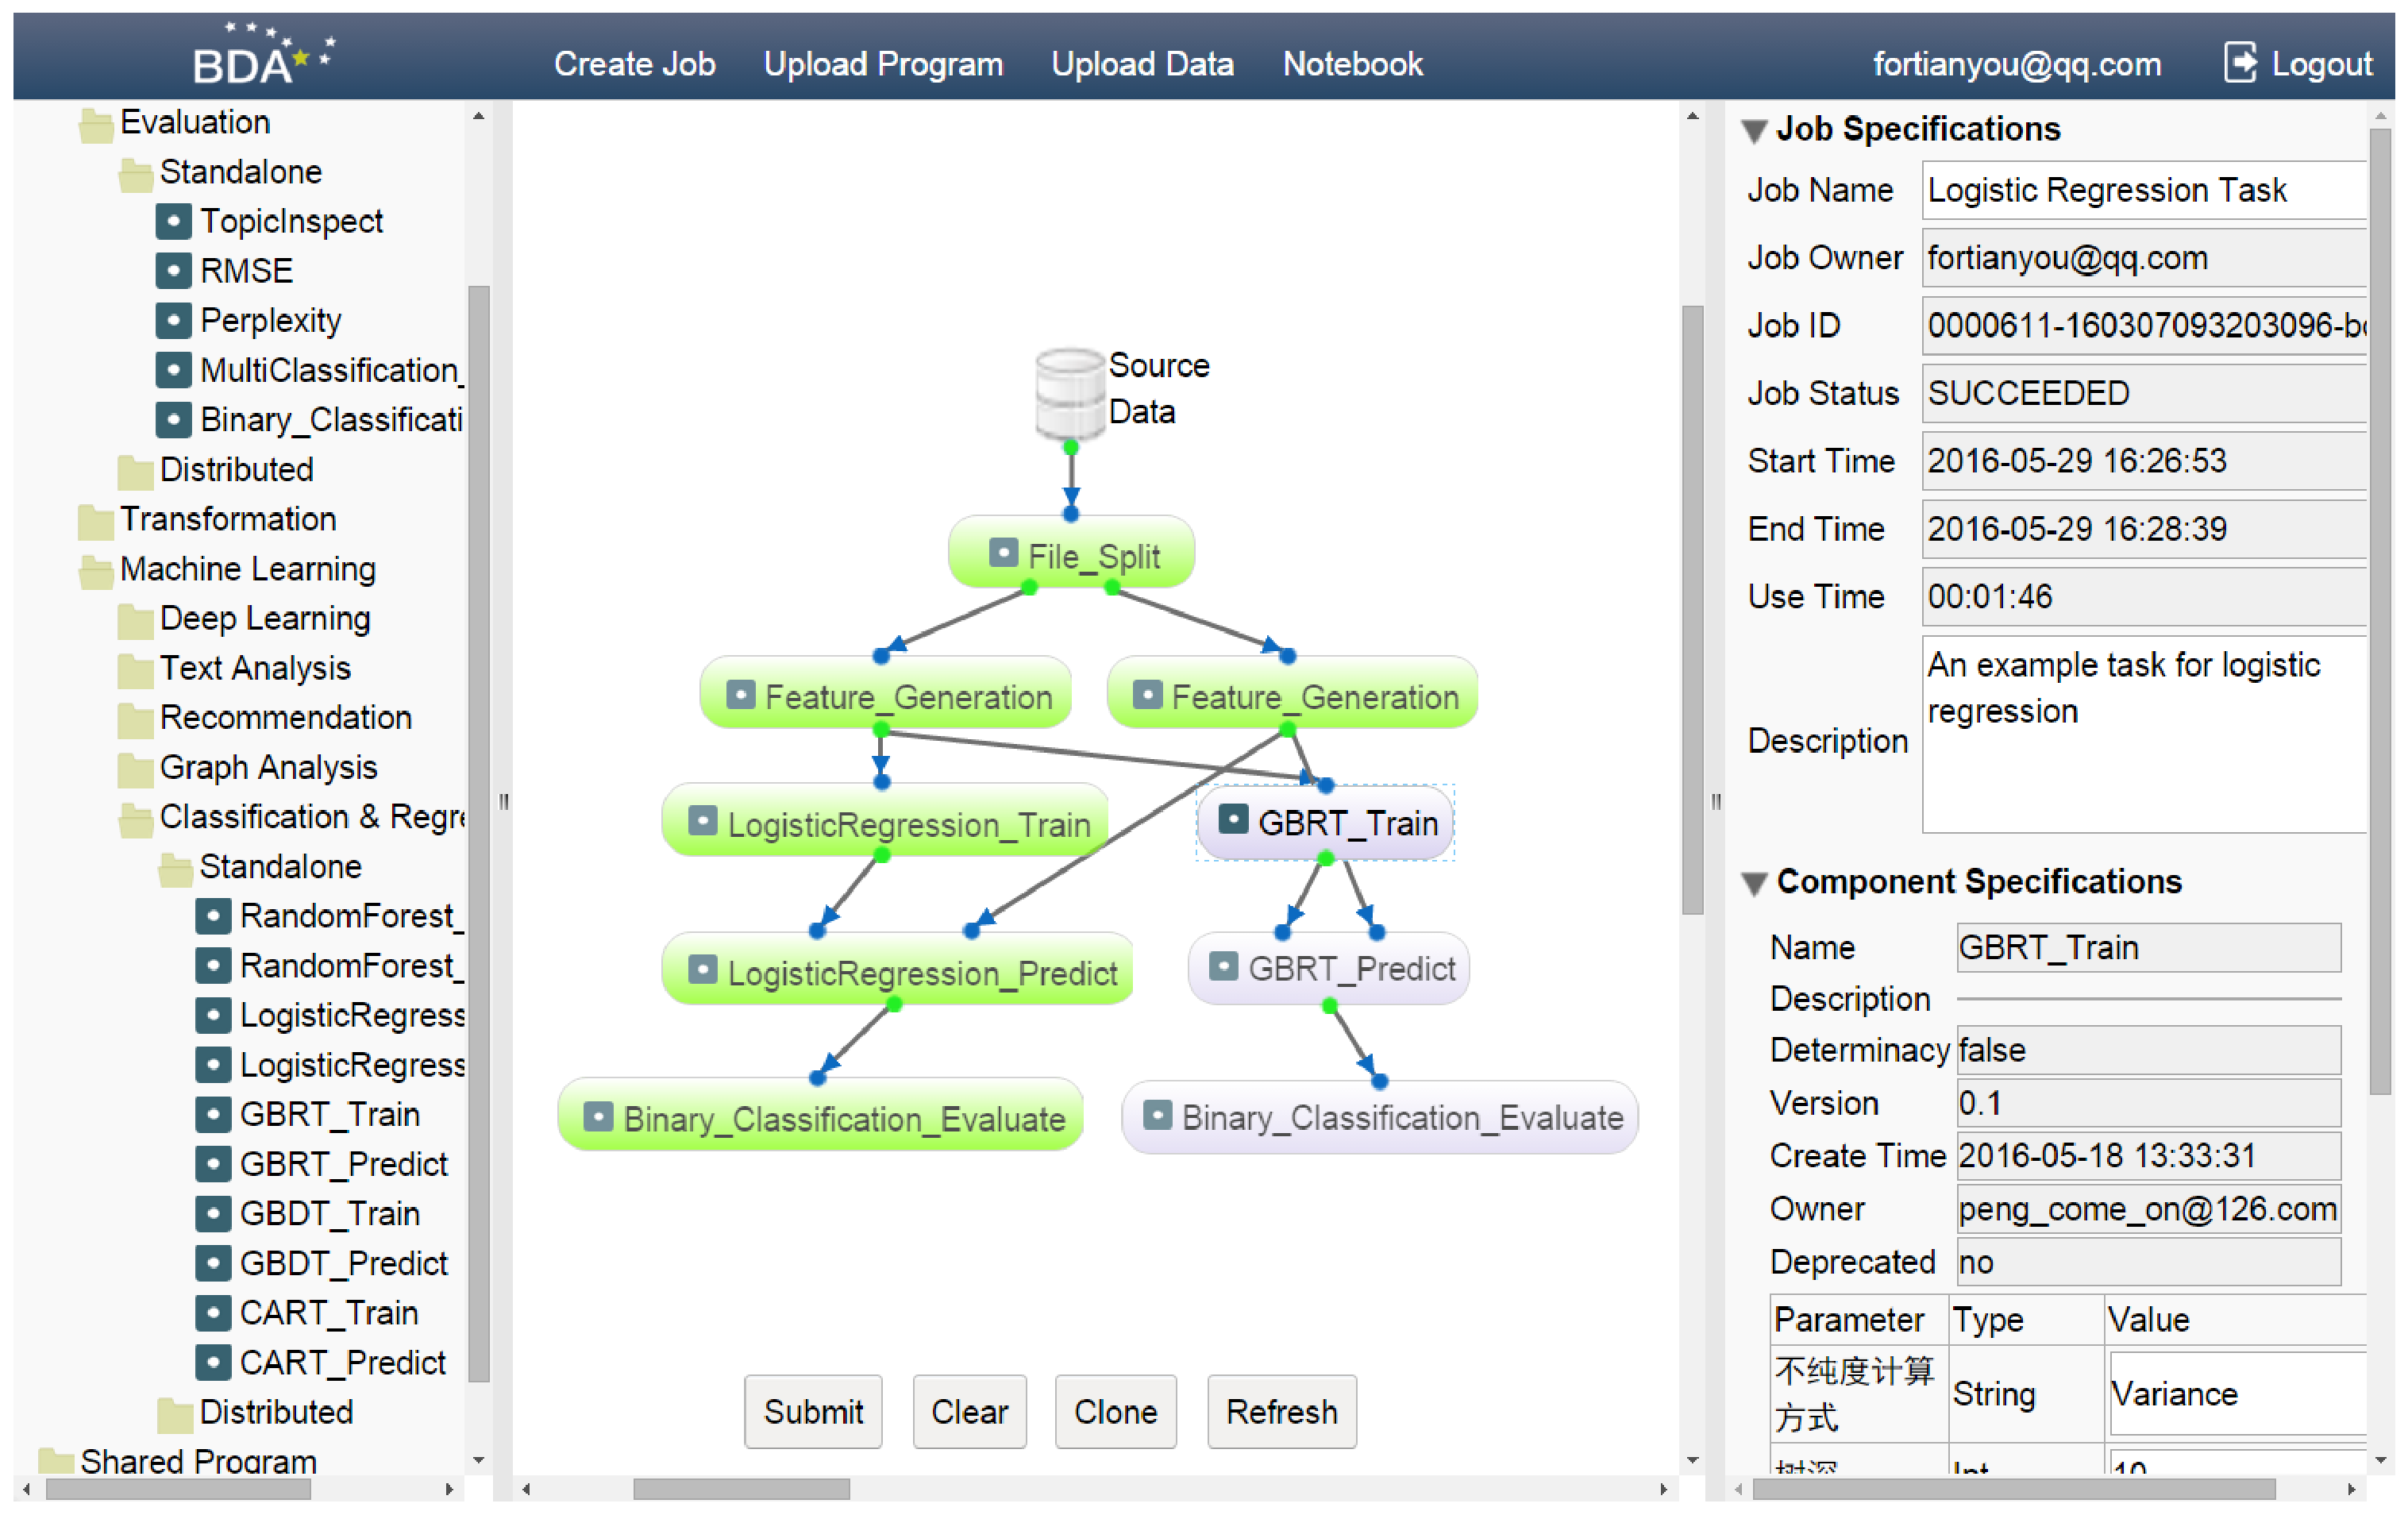
\includegraphics[width = 0.4\textwidth]{job_reuse.eps}
\end{figure}

Submit the job again, the node which had been finished would be skipped. and the result output data would be reused for the new operations.

\begin{figure}[!htb]
\centering
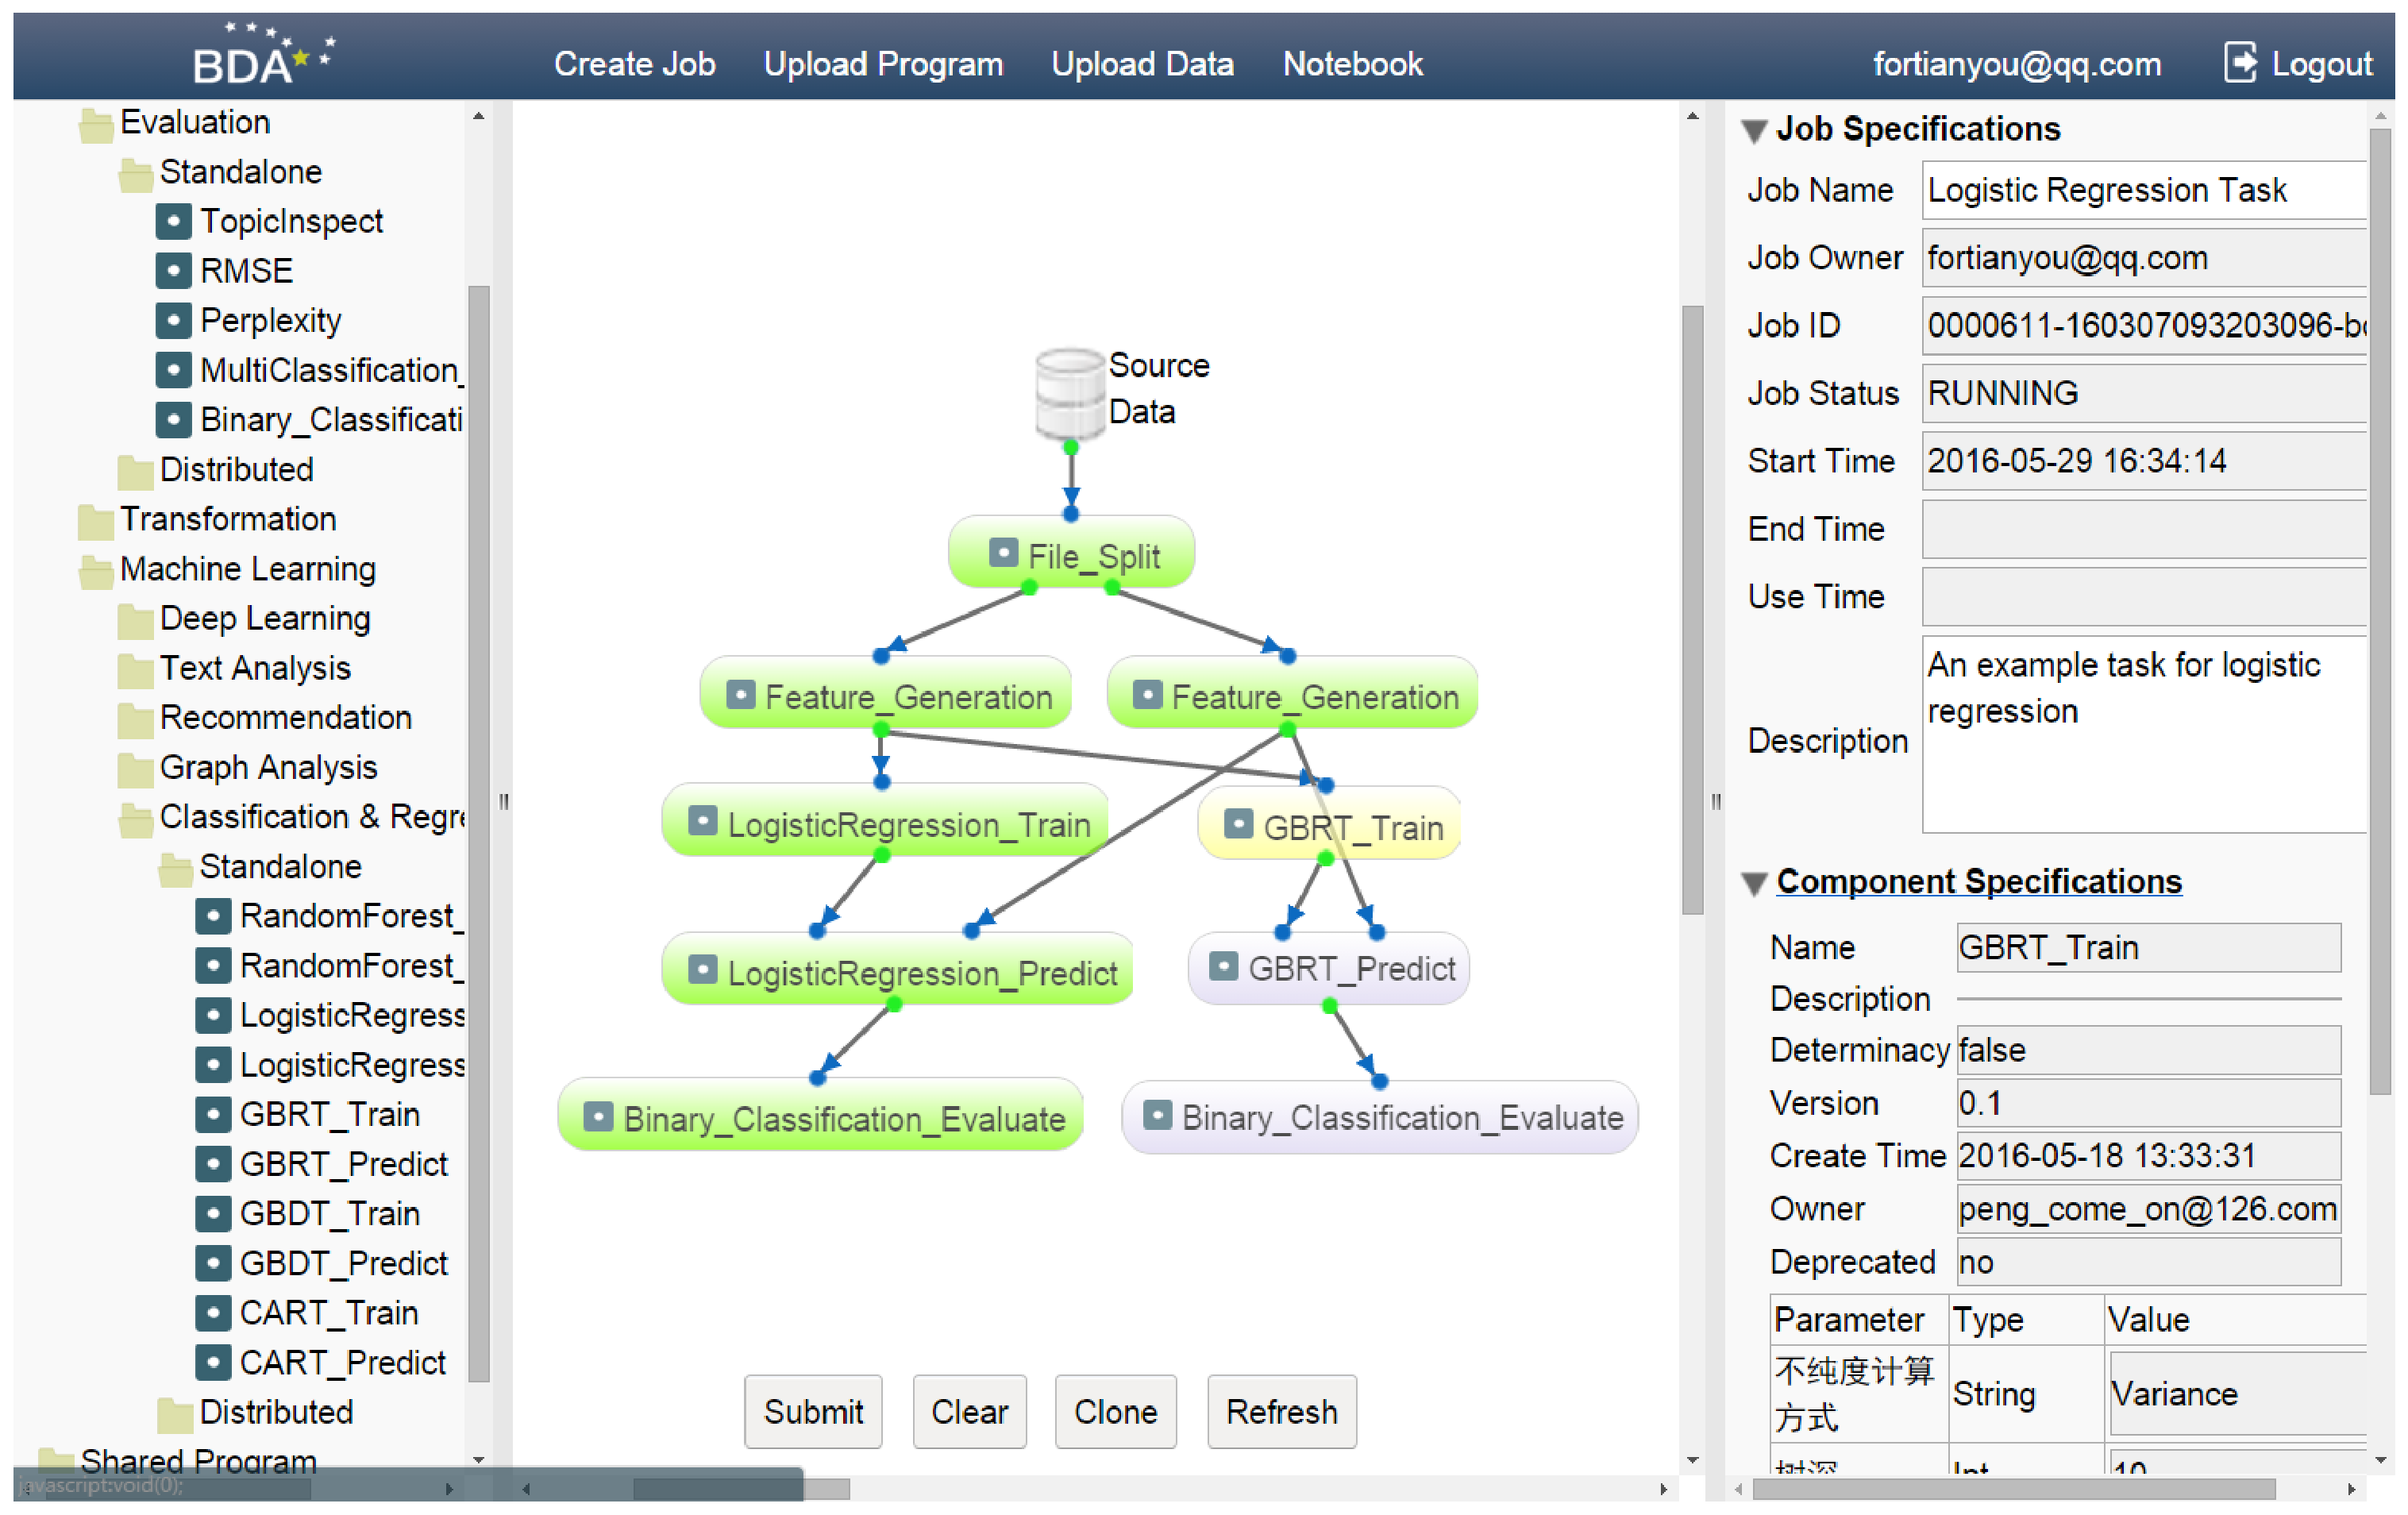
\includegraphics[width = 0.4\textwidth]{job_reuse_submit.eps}
\end{figure}

Finally, one could have a sight on the job at anytime/anywhere through the URL respect to the job.
\begin{figure}[!htb]
\centering
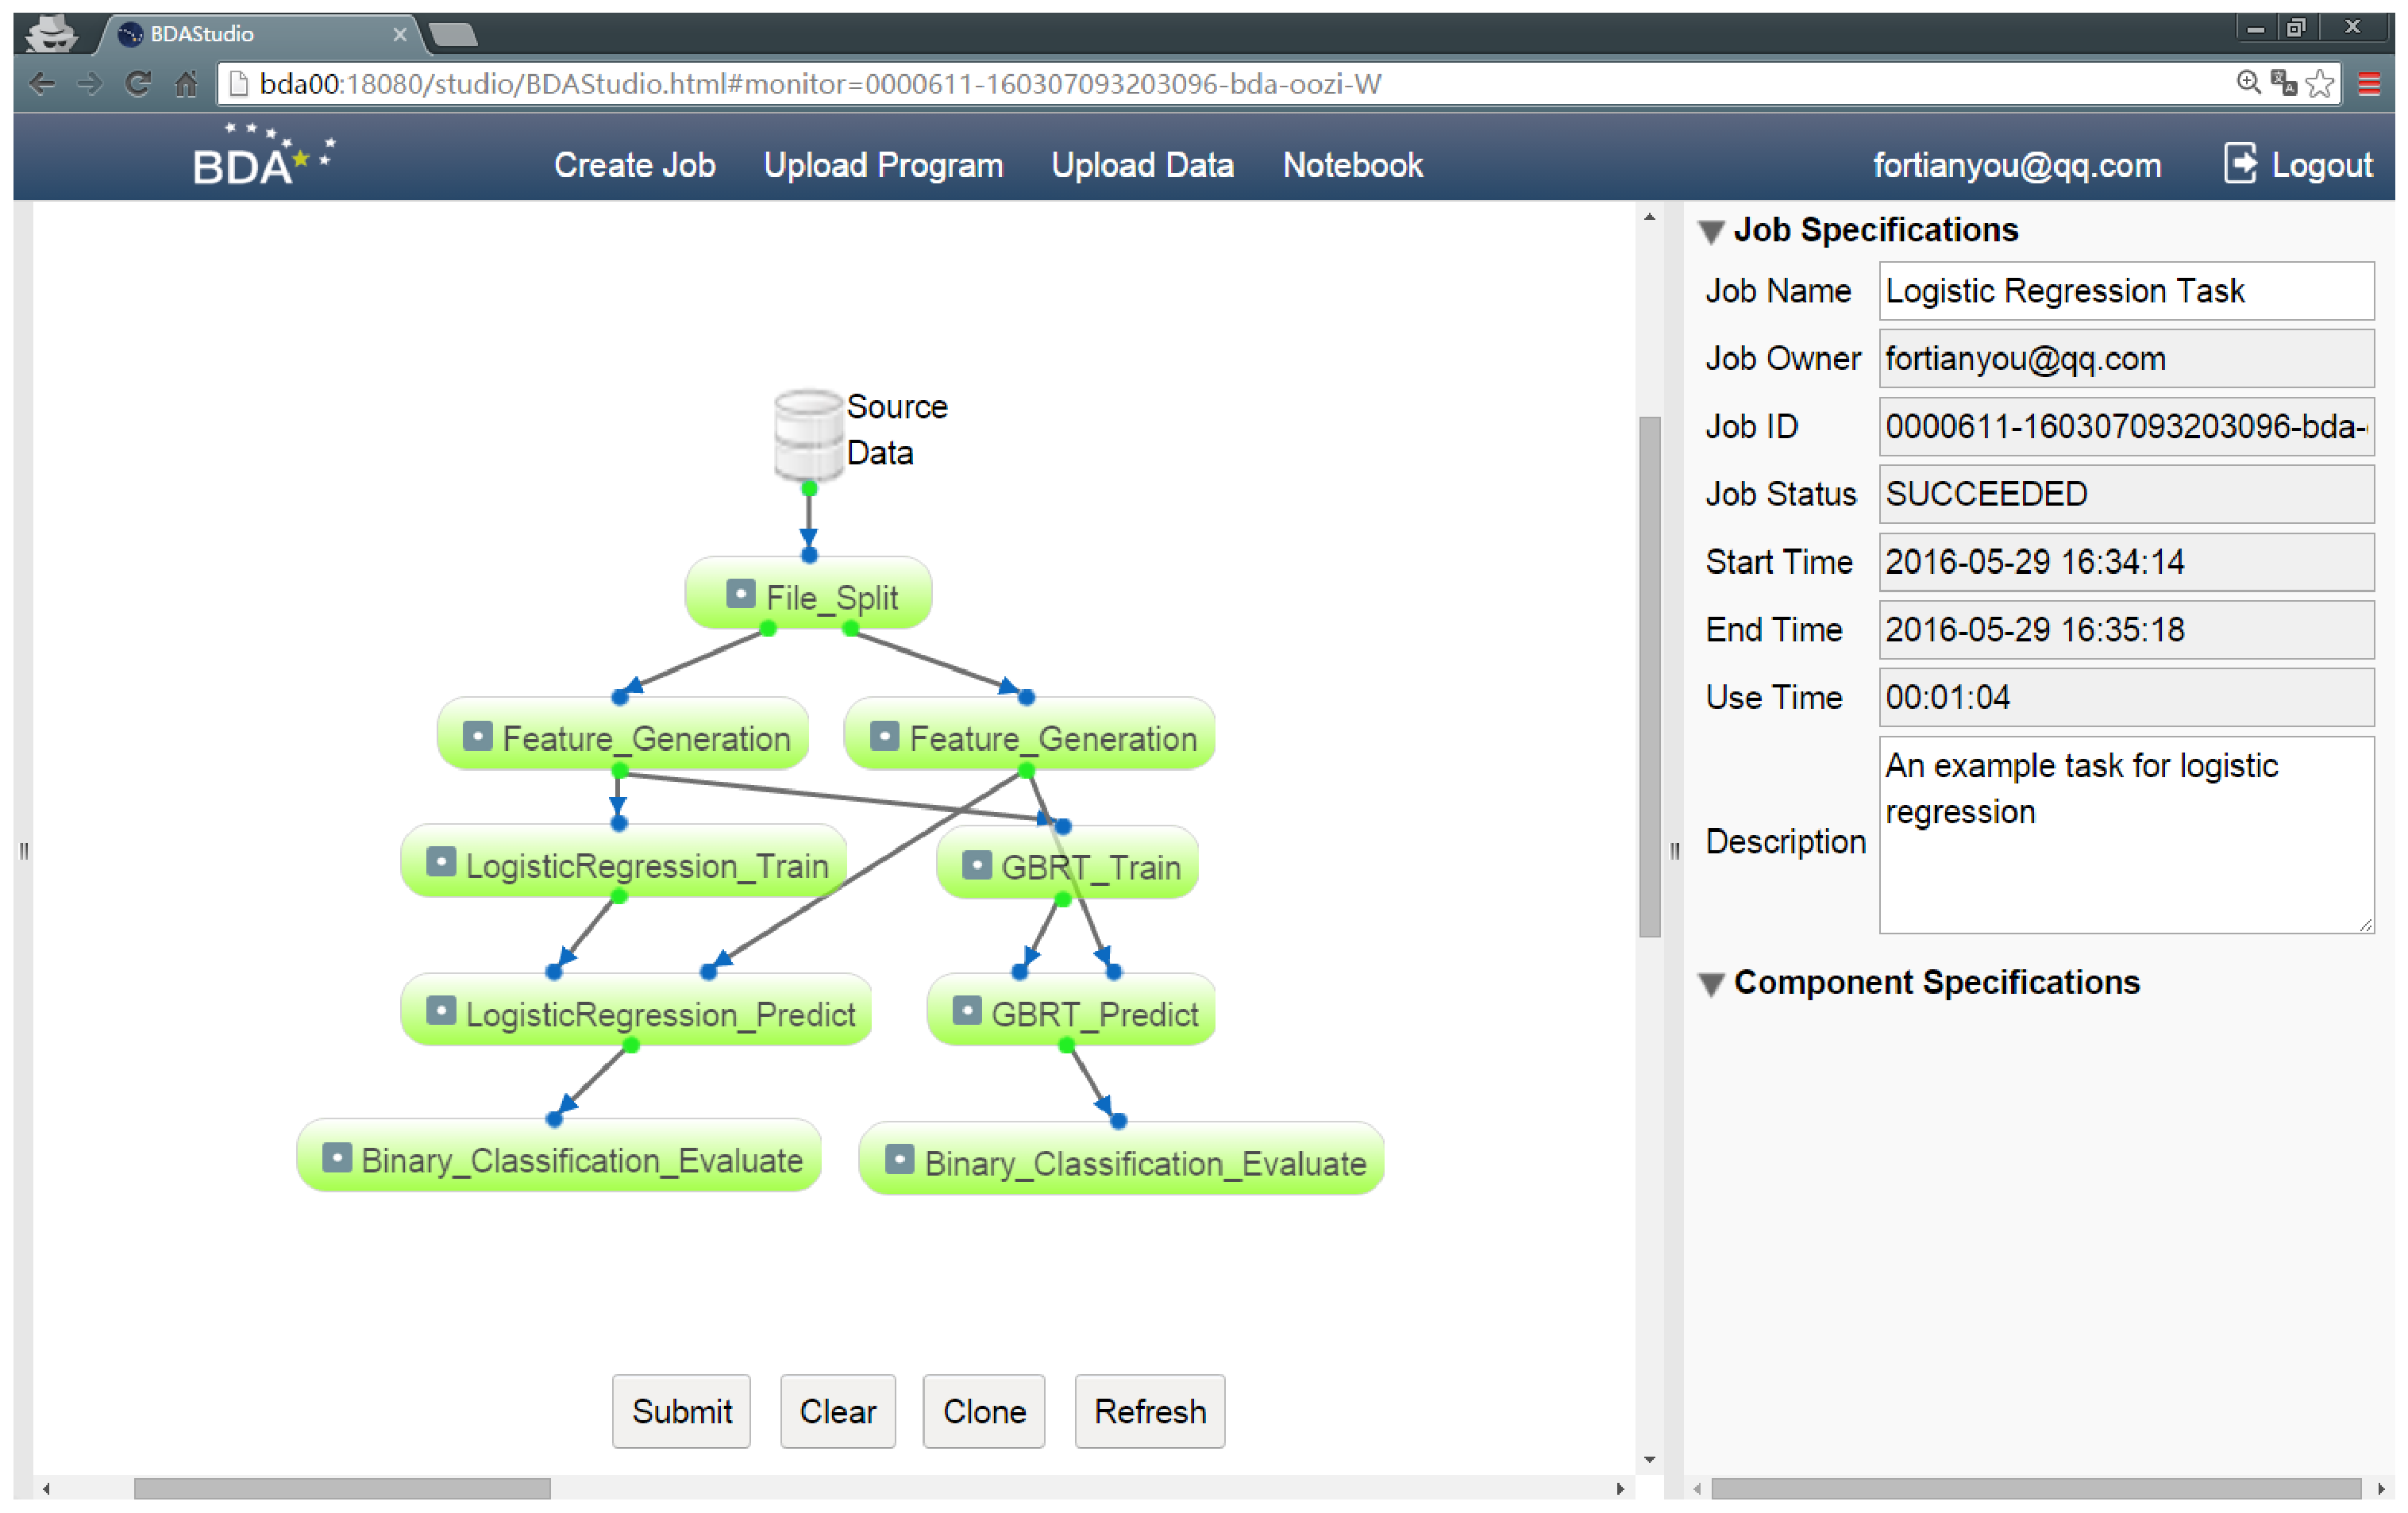
\includegraphics[width = 0.4\textwidth]{job_view.eps}
\end{figure}

\noindent\textbf{Program Upload Panel}

We support program upload and semi-auto command line format generation by the panel bellow, where the basic informations are on the left, command line format configuration region on the right, and program package upload region on the bottom:

\begin{figure}[!htb]
\centering
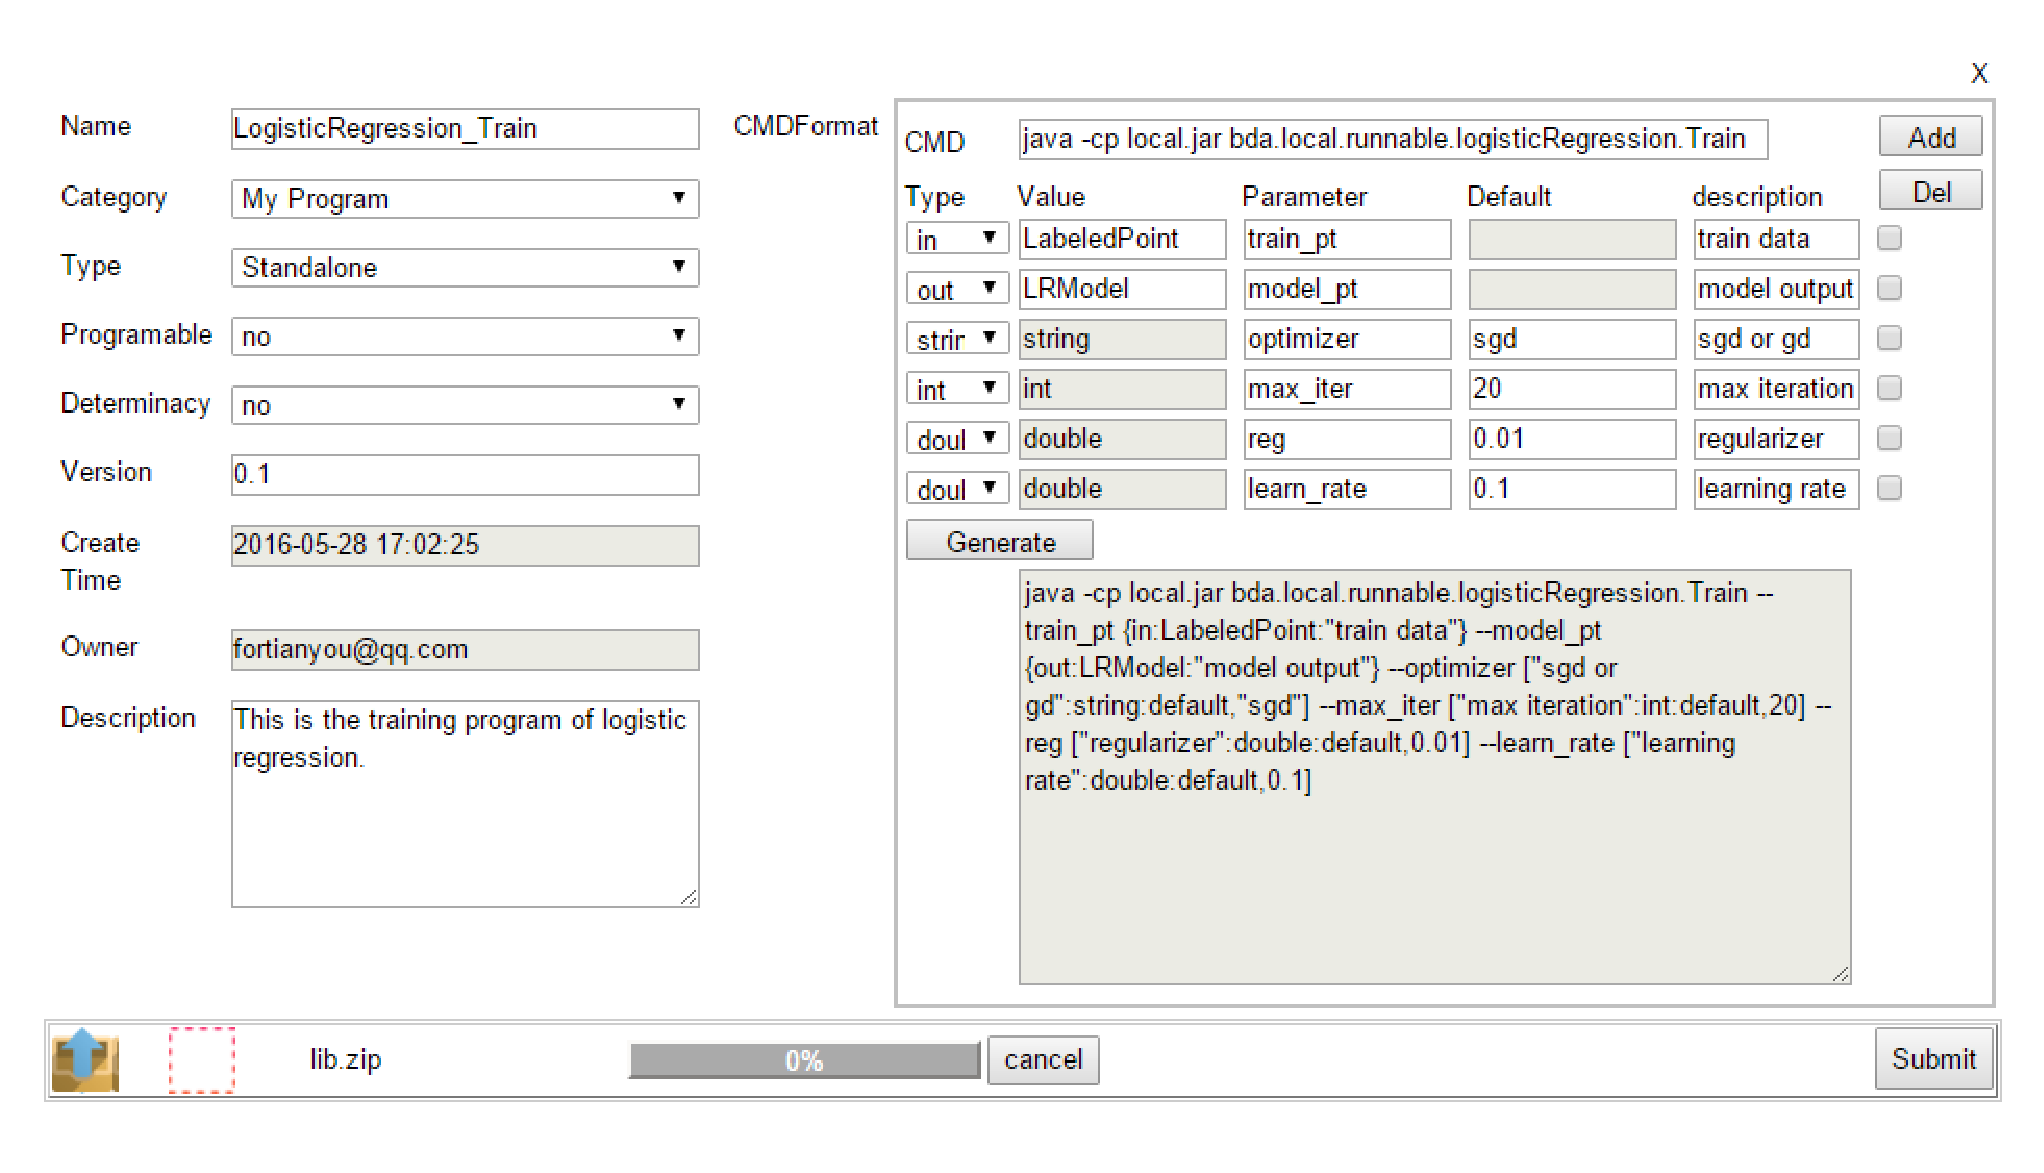
\includegraphics[width = 0.4\textwidth]{Upload_Program.eps}
\end{figure}


\end{document}
